\documentclass[10pt,journal,compsoc]{IEEEtran}

\usepackage{graphicx}
\usepackage{amsmath,amssymb,amsthm}
\usepackage{booktabs}
\usepackage{tikz}
\usepackage{enumitem}
\usepackage{url}
\usepackage{cite}
\usepackage{xcolor}
\usepackage{colortbl}
\usepackage{multirow}
\usepackage{array}
\usetikzlibrary{shapes,arrows,positioning,fit,backgrounds,calc,decorations.pathreplacing,arrows.meta}

\newcommand{\yonakh}{\textsc{Yonakh}}

\definecolor{headerblue}{RGB}{41,65,114}
\definecolor{lightgray}{RGB}{245,245,245}
\definecolor{medgray}{RGB}{220,220,220}

\newtheorem{definition}{Definition}

\begin{document}

\title{Yonakh: A Shared Memory Architecture for Multi-Agent AI-Assisted Software Development}

\author{Shashank Venkat\\
\textit{shashyv@gmail.com}}

\IEEEtitleabstractindextext{%
\begin{abstract}
The proliferation of AI coding assistants---Claude Code, Cursor, GitHub Copilot, and OpenAI Codex---is transforming software development practice. However, each tool maintains isolated, ephemeral memory: architecture decisions recorded in one session are invisible to another; failed debugging attempts are repeated across tools; design rationale evaporates between conversations. This \emph{memory fragmentation} undermines the potential of AI-assisted development and contributes to organizational knowledge loss.

We present \yonakh, a local-first, vendor-neutral memory server that provides a shared knowledge layer for heterogeneous AI coding assistants. \yonakh\ models software engineering knowledge as a typed knowledge graph with 21 entity types (decisions, bugs, failed attempts, design rationale, commits, etc.) and 21 relationship types (supersedes, contradicts, implements, reverts, etc.). A memory quality engine manages knowledge lifecycle through multi-signal importance scoring, temporal decay with domain-specific half-lives, and automated conflict detection. Hybrid search combining full-text and semantic retrieval via Reciprocal Rank Fusion enables effective knowledge recall.

We contribute: (1) a formal ontology for software engineering knowledge in AI-assisted development; (2) a memory quality model addressing knowledge staleness and contradiction; (3) an open architecture enabling memory interoperability via REST API and Model Context Protocol (MCP); and (4) a theoretical justification grounded in cognitive science for why shared memory improves AI-assisted development outcomes.
\end{abstract}

\begin{IEEEkeywords}
AI coding assistants, knowledge graphs, software engineering knowledge management, LLM agents, memory systems, Model Context Protocol
\end{IEEEkeywords}}

\maketitle

\IEEEdisplaynontitleabstractindextext
\IEEEpeerreviewmaketitle

\section{Introduction}
\IEEEPARstart{A}{rtificial} intelligence is reshaping software development at an unprecedented pace. AI coding assistants---including Anthropic's Claude Code, Cursor, GitHub Copilot, and OpenAI Codex---now participate in millions of coding sessions daily, providing assistance with code generation, debugging, refactoring, documentation, and architectural decision-making \cite{vaithilingam2022expectation,barke2023grounded}. Industry surveys indicate that over 70\% of professional developers now use AI coding tools regularly, with many reporting significant productivity improvements \cite{github2023survey}.

Yet beneath these productivity gains lies a fundamental limitation: \emph{memory fragmentation}. Each AI tool maintains its own isolated context, typically bounded by conversation windows or session limits. This isolation creates concrete problems:

\begin{enumerate}
\item \textbf{Cross-tool invisibility:} When a developer records an architecture decision with Claude Code, that knowledge remains invisible to Cursor. Each tool operates in its own epistemic bubble.

\item \textbf{Session amnesia:} When a debugging session concludes, the root cause analysis, attempted solutions, and lessons learned typically vanish. The next session starts from scratch.

\item \textbf{Repeated mistakes:} When one team member discovers that a particular approach fails, there is no mechanism for that negative knowledge to persist and prevent others from repeating the mistake.

\item \textbf{Lost rationale:} Architecture decisions accumulate in code, but the reasoning behind them---the alternatives considered, the constraints that drove the choice---evaporates with each session's end.

\item \textbf{Onboarding friction:} New team members cannot access the accumulated wisdom of past sessions. Every participant starts with a blank slate.
\end{enumerate}

Prior research on turnover-induced knowledge loss demonstrates that departing developers take irreplaceable tacit knowledge with them, reducing productivity and increasing defects \cite{rigby2016quantifying,nassif2021turnover}. AI assistants amplify this: they generate knowledge at unprecedented rates but lack any mechanism for persistence, sharing, or quality management. The result is \emph{collective amnesia} where valuable engineering knowledge is continuously created and lost.

This paper introduces \yonakh, a shared memory architecture for multi-agent AI-assisted software development. Our contributions are:

\begin{enumerate}
\item A \textbf{domain ontology} comprising 21 entity types and 21 relationship types for software engineering knowledge.

\item A \textbf{memory quality model} formalizing knowledge lifecycle through importance scoring, temporal decay, and conflict detection.

\item An \textbf{open architecture} enabling memory interoperability via REST and Model Context Protocol (MCP).

\item A \textbf{theoretical justification} grounded in cognitive science and knowledge management theory.
\end{enumerate}

This paper presents an architectural vision and framework; empirical evaluation of the system's impact on developer productivity and knowledge retention remains future work.

\section{Background and Related Work}

\subsection{Architecture Decision Records}

The challenge of capturing architectural decisions has long been recognized. Kruchten et al. \cite{kruchten2006decision} introduced architectural knowledge management, arguing that decisions deserve first-class treatment. Nygard \cite{nygard2011adr} operationalized this through Architecture Decision Records (ADRs): lightweight documents capturing decisions with context and consequences.

Recent studies validate ADRs' effectiveness. Soldani et al. \cite{soldani2024adr} found ADRs improve documentation culture and knowledge transfer, though they struggle with distributed systems. Practitioners express concerns about documentation burden and keeping records current \cite{tofan2023adr,zimmermann2015architectural}.

\yonakh\ addresses these limitations by expanding beyond decisions to 21 entity types, adding relationship modeling, introducing temporal dynamics, and providing machine interfaces enabling AI tools to create records automatically.

\subsection{Knowledge Graphs in Software Engineering}

Recent work integrates knowledge graphs with LLMs for code understanding. CodexGraph \cite{liu2024codexgraph} bridges LLMs and repositories through graph databases, enabling multi-hop reasoning over code structure. Similar approaches incorporate graph structures into retrieval and attention mechanisms for repository-level tasks.

These approaches focus on \emph{code structure}. \yonakh\ complements them by modeling \emph{meta-knowledge}: decisions, rationale, and lessons learned that surround code.

\subsection{Memory Systems for LLM Agents}

Memory management is critical for LLM agents. Park et al. \cite{park2023generative} introduced memory streams with reflection for generative agents, demonstrating how retrieval-augmented memory enables coherent long-term behavior. Subsequent work has explored hierarchical memory architectures that decompose storage into working, episodic, and semantic tiers, mirroring human cognitive systems \cite{baddeley2012working}. Other approaches treat context management as an explicit tool that agents can invoke to manage their own memory constraints.

These optimize memory \emph{within} a single agent. \yonakh\ addresses memory \emph{across} agents and tools---enabling multiple AI assistants to share a knowledge substrate.

\subsection{Organizational Knowledge Loss}

Software engineering research documents significant impacts from knowledge loss. Rigby et al. \cite{rigby2016quantifying} found projects susceptible to losses three times larger than expected. Nassif and Robillard \cite{nassif2021turnover} identified challenges across culture, tacit knowledge, documentation, and tools.

AI assistants create a new dimension: they generate knowledge at scale but it exists only in ephemeral conversation logs. \yonakh\ provides infrastructure to capture this knowledge as organizational memory.

\section{Theoretical Foundation}

Why should shared, quality-aware memory improve AI-assisted development? We ground \yonakh's design in cognitive science and knowledge management theory.

\subsection{Cognitive Architecture Parallels}

Human cognition relies on multiple memory systems \cite{baddeley2012working,tulving1985memory}: working memory (limited capacity, immediate processing), episodic memory (specific events), semantic memory (general knowledge), and procedural memory (skills).

Current AI assistants have severely constrained working memory (context windows) and no persistent long-term memory across sessions. This is equivalent to a developer with complete anterograde amnesia---able to reason about immediate context but unable to form new long-term memories.

\yonakh\ provides the missing systems:
\begin{itemize}
\item \textbf{Entity storage} parallels episodic memory
\item \textbf{Relationship graph} parallels semantic memory
\item \textbf{Rules engine} parallels procedural memory
\end{itemize}

\subsection{Knowledge Management Theory}

Nonaka and Takeuchi's SECI model \cite{nonaka1995knowledge} describes knowledge creation through Socialization, Externalization, Combination, and Internalization. AI assistants participate in Externalization and Combination but without persistent memory, outputs are lost.

Wegner's transactive memory \cite{wegner1987transactive} describes how groups distribute cognitive labor---members know \emph{who knows what}. Current AI tools cannot participate because their knowledge is inaccessible. \yonakh\ enables AI tools to contribute to the team's transactive memory system.

\subsection{Formal Model of Memory Effectiveness}

We formalize the value of shared memory. Let $\mathcal{K}_t$ denote the knowledge state at time $t$, and let $\mathcal{A} = \{a_1, \ldots, a_n\}$ be a set of AI agents. Without shared memory, each agent maintains isolated state:
\begin{equation}
\mathcal{K}_t^{(i)} \cap \mathcal{K}_t^{(j)} = \emptyset \quad \forall i \neq j
\end{equation}

With \yonakh, agents share a common substrate:
\begin{equation}
\mathcal{K}_t^{\text{shared}} = \bigcup_{i=1}^{n} \mathcal{K}_t^{(i)}
\end{equation}

The information gain for agent $a_i$ accessing shared memory is:
\begin{equation}
\Delta\mathcal{I}_i = H(\mathcal{K}_t^{\text{shared}}) - H(\mathcal{K}_t^{(i)})
\end{equation}
where $H(\cdot)$ denotes entropy. This formalizes how agents benefit from knowledge they did not generate.

\section{The Yonakh Architecture}

\yonakh\ is implemented as a local server providing REST API and MCP interfaces to a SQLite-based knowledge store. Fig.~\ref{fig:architecture} illustrates the high-level architecture.

\begin{figure}[t]
\centering
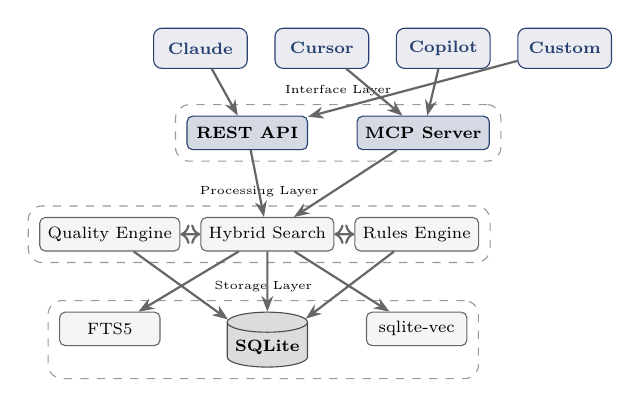
\begin{tikzpicture}[
    scale=0.85,
    transform shape,
    node distance=0.4cm and 0.6cm,
    agent/.style={rectangle, draw=headerblue, fill=headerblue!10, rounded corners=3pt, minimum width=1.4cm, minimum height=0.6cm, font=\scriptsize\bfseries, text=headerblue},
    api/.style={rectangle, draw=headerblue, fill=headerblue!20, rounded corners=2pt, minimum width=1.8cm, minimum height=0.5cm, font=\scriptsize\bfseries},
    component/.style={rectangle, draw=black!60, fill=lightgray, rounded corners=2pt, minimum width=1.5cm, minimum height=0.5cm, font=\scriptsize},
    db/.style={cylinder, draw=black!70, fill=medgray, shape border rotate=90, aspect=0.25, minimum height=0.7cm, minimum width=1.2cm, font=\scriptsize\bfseries},
    arrow/.style={-{Stealth[length=2mm]}, thick, draw=black!60}
]

\node[agent] (claude) {Claude};
\node[agent, right=0.4cm of claude] (cursor) {Cursor};
\node[agent, right=0.4cm of cursor] (copilot) {Copilot};
\node[agent, right=0.4cm of copilot] (custom) {Custom};

\node[api, below=0.7cm of claude, xshift=0.7cm] (rest) {REST API};
\node[api, below=0.7cm of copilot, xshift=-0.3cm] (mcp) {MCP Server};

\node[draw=black!40, dashed, rounded corners=5pt, fit=(rest)(mcp), inner sep=4pt, label={[font=\tiny]above:Interface Layer}] (iface) {};

\node[component, below=1.0cm of rest, xshift=0.3cm] (search) {Hybrid Search};
\node[component, left=0.3cm of search] (quality) {Quality Engine};
\node[component, right=0.3cm of search] (rules) {Rules Engine};

\node[draw=black!40, dashed, rounded corners=5pt, fit=(quality)(search)(rules), inner sep=4pt, label={[font=\tiny]above:Processing Layer}] (proc) {};

\node[component, below=0.9cm of quality] (fts) {FTS5};
\node[db, below=0.9cm of search] (sqlite) {SQLite};
\node[component, below=0.9cm of rules] (vec) {sqlite-vec};

\node[draw=black!40, dashed, rounded corners=5pt, fit=(fts)(sqlite)(vec), inner sep=4pt, label={[font=\tiny]above:Storage Layer}] (store) {};

\draw[arrow] (claude) -- (rest);
\draw[arrow] (cursor) -- (mcp);
\draw[arrow] (copilot) -- (mcp);
\draw[arrow] (custom) -- (rest);

\draw[arrow] (rest) -- (search);
\draw[arrow] (mcp) -- (search);

\draw[arrow, <->] (search) -- (quality);
\draw[arrow, <->] (search) -- (rules);

\draw[arrow] (quality) -- (sqlite);
\draw[arrow] (search) -- (fts);
\draw[arrow] (search) -- (sqlite);
\draw[arrow] (search) -- (vec);
\draw[arrow] (rules) -- (sqlite);

\end{tikzpicture}
\caption{Three-layer architecture of \yonakh. AI agents connect through REST or MCP interfaces. The processing layer handles search, quality scoring, and rule inference. The storage layer combines full-text (FTS5), relational (SQLite), and vector (sqlite-vec) capabilities.}
\label{fig:architecture}
\end{figure}

\subsection{Knowledge Graph Ontology}

\begin{definition}[Knowledge Graph]
The \yonakh\ knowledge graph is a labeled property graph $G = (V, E, \tau_V, \tau_E, \phi)$ where:
\begin{itemize}
\item $V$ is the set of entity vertices
\item $E \subseteq V \times V$ is the set of directed edges
\item $\tau_V: V \to \mathcal{T}_V$ assigns entity types from $|\mathcal{T}_V| = 21$ types
\item $\tau_E: E \to \mathcal{T}_E$ assigns relationship types from $|\mathcal{T}_E| = 21$ types
\item $\phi: V \cup E \to \mathcal{P}$ assigns property maps
\end{itemize}
\end{definition}

Table~\ref{tab:entities} presents the entity taxonomy, and Table~\ref{tab:relationships} presents the relationship taxonomy.

\begin{table}[t]
\caption{Entity Types in the \yonakh\ Knowledge Graph Ontology}
\label{tab:entities}
\centering
\small
\renewcommand{\arraystretch}{1.3}
\begin{tabular}{@{}p{0.22\columnwidth} p{0.70\columnwidth}@{}}
\toprule
\textbf{Category} & \textbf{Entity Types} \\
\midrule
Version Control & commit, branch, pull\_request, code\_review, issue \\
Decisions & decision, design\_rationale, failed\_attempt, bug\_report \\
Communication & conversation, message, meeting\_note, slack\_thread \\
Artifacts & document, snippet, benchmark, experiment \\
Organization & person, project, component, concept \\
\bottomrule
\end{tabular}
\end{table}

\begin{table}[t]
\caption{Relationship Types by Semantic Category}
\label{tab:relationships}
\centering
\small
\renewcommand{\arraystretch}{1.3}
\begin{tabular}{@{}p{0.18\columnwidth} p{0.74\columnwidth}@{}}
\toprule
\textbf{Category} & \textbf{Relationship Types} \\
\midrule
Causal & caused\_by, resulted\_in, triggered \\
Structural & part\_of, depends\_on, contains, derived\_from \\
Epistemic & contradicts, supersedes, reverts, validates \\
Social & authored\_by, reviewed\_by, assigned\_to, mentioned \\
Reference & modifies, references, documented\_in, implements \\
\bottomrule
\end{tabular}
\end{table}

Fig.~\ref{fig:knowledge-graph} illustrates a sample knowledge graph fragment showing interconnected entities.

\begin{figure}[t]
\centering
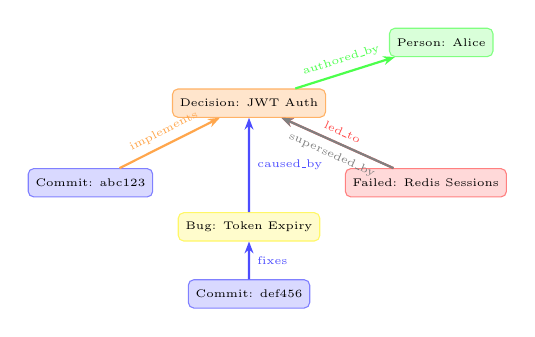
\begin{tikzpicture}[
    scale=0.8,
    transform shape,
    node distance=1.2cm,
    entity/.style={rectangle, draw, rounded corners=2pt, minimum width=1.2cm, minimum height=0.45cm, font=\tiny},
    decision/.style={entity, fill=orange!20, draw=orange!60},
    commit/.style={entity, fill=blue!15, draw=blue!50},
    failed/.style={entity, fill=red!15, draw=red!50},
    bug/.style={entity, fill=yellow!20, draw=yellow!60},
    person/.style={entity, fill=green!15, draw=green!50},
    edge/.style={-{Stealth[length=1.5mm]}, thick, font=\tiny},
]

\node[decision] (d1) {Decision: JWT Auth};
\node[commit, below left=0.8cm and 0.3cm of d1] (c1) {Commit: abc123};
\node[failed, below right=0.8cm and 0.3cm of d1] (f1) {Failed: Redis Sessions};
\node[bug, below=1.5cm of d1] (b1) {Bug: Token Expiry};
\node[person, above right=0.5cm and 1cm of d1] (p1) {Person: Alice};
\node[commit, below=0.6cm of b1] (c2) {Commit: def456};

\draw[edge, orange!70] (c1) -- node[above, sloped] {implements} (d1);
\draw[edge, red!70] (f1) -- node[above, sloped] {led\_to} (d1);
\draw[edge, blue!70] (b1) -- node[right] {caused\_by} (d1);
\draw[edge, green!70] (d1) -- node[above, sloped] {authored\_by} (p1);
\draw[edge, blue!70] (c2) -- node[right] {fixes} (b1);
\draw[edge, gray] (f1) -- node[below, sloped] {superseded\_by} (d1);

\end{tikzpicture}
\caption{Sample knowledge graph fragment. A decision entity connects to its implementation commit, the failed attempt it replaced, bugs it caused, and its author. Edge colors indicate relationship categories.}
\label{fig:knowledge-graph}
\end{figure}

\subsection{Memory Quality Model}

Knowledge relevance is not static. \yonakh\ formalizes quality through importance scoring, temporal decay, and conflict detection.

\subsubsection{Importance Scoring}

\begin{definition}[Importance Function]
The importance $I: V \to [0,1]$ of an entity $e \in V$ is a weighted combination of five signals:
\begin{equation}
I(e) = \sum_{s \in \mathcal{S}} w_s \cdot \sigma_s(e)
\end{equation}
where $\mathcal{S} = \{T, C, A, R, X\}$ are the signal types and $\sum_{s} w_s = 1$.
\end{definition}

The individual signals are computed as follows:

\textbf{Type Signal} $T(e)$: Intrinsic importance based on entity type:
\begin{equation}
T(e) = \begin{cases}
0.9 & \text{if } \tau_V(e) \in \{\texttt{decision}\} \\
0.8 & \text{if } \tau_V(e) \in \{\texttt{bug\_report}, \texttt{design\_rationale}\} \\
0.7 & \text{if } \tau_V(e) \in \{\texttt{failed\_attempt}\} \\
0.5 & \text{if } \tau_V(e) \in \{\texttt{pull\_request}, \texttt{issue}\} \\
0.3 & \text{otherwise}
\end{cases}
\end{equation}

\textbf{Connectivity Signal} $C(e)$: Graph centrality normalized by maximum degree:
\begin{equation}
C(e) = \frac{\deg^+(e) + \deg^-(e)}{\max_{v \in V}(\deg^+(v) + \deg^-(v))}
\end{equation}

\textbf{Access Signal} $A(e)$: Recency-weighted access frequency:
\begin{equation}
A(e) = \frac{1}{Z} \sum_{i=1}^{n} \exp\left(-\lambda \cdot \Delta t_i\right)
\end{equation}
where $\Delta t_i$ is time since access $i$, $\lambda = 0.1$ day$^{-1}$, and $Z$ normalizes to $[0,1]$.

\textbf{Richness Signal} $R(e)$: Content completeness:
\begin{equation}
R(e) = \alpha \cdot \mathbb{1}[|\text{content}| > \theta_c] + \beta \cdot \frac{|\phi(e)|}{\theta_p} + \gamma \cdot \mathbb{1}[\text{has\_tags}]
\end{equation}
with $\alpha = 0.4$, $\beta = 0.4$, $\gamma = 0.2$.

\textbf{Explicit Signal} $X(e)$: User-provided importance override.

Table~\ref{tab:weights} shows the signal weights used in production.

\begin{table}[t]
\caption{Importance Signal Weights}
\label{tab:weights}
\centering
\small
\renewcommand{\arraystretch}{1.3}
\begin{tabular}{@{}p{0.55\columnwidth} c r@{}}
\toprule
\textbf{Signal} & \textbf{Sym.} & \textbf{Wt.} \\
\midrule
Type (intrinsic value) & $w_T$ & 0.30 \\
Explicit (user override) & $w_X$ & 0.30 \\
Connectivity (graph centrality) & $w_C$ & 0.15 \\
Access (usage frequency) & $w_A$ & 0.15 \\
Richness (content completeness) & $w_R$ & 0.10 \\
\bottomrule
\end{tabular}
\end{table}

\subsubsection{Temporal Decay}

Knowledge relevance decreases over time at rates varying by entity type. We model decay with a sigmoid function:

\begin{definition}[Decay Function]
The temporal decay $D: V \times \mathbb{R}^+ \to [0,1]$ is:
\begin{equation}
D(e, t) = \frac{1}{1 + \exp\left(\frac{\text{age}(e, t) - h(\tau_V(e))}{k \cdot h(\tau_V(e))}\right)}
\end{equation}
where $\text{age}(e,t) = t - t_{\text{created}}(e)$, $h(\cdot)$ is the type-specific half-life, and $k = 0.2$ controls steepness.
\end{definition}

Fig.~\ref{fig:decay-curves} visualizes decay curves for different entity types, and Table~\ref{tab:halflife} lists the half-life values.

\begin{figure}[t]
\centering
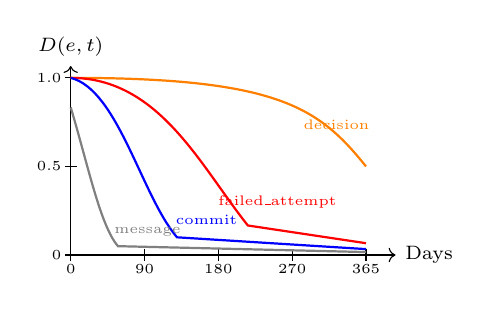
\begin{tikzpicture}[scale=0.75]
\begin{scope}
\draw[->] (0,0) -- (5.5,0) node[right, font=\scriptsize] {Days};
\draw[->] (0,0) -- (0,3.2) node[above, font=\scriptsize] {$D(e,t)$};

\foreach \y/\label in {0/0, 1.5/0.5, 3/1.0} {
  \draw (-0.1,\y) -- (0.1,\y) node[left, font=\tiny, xshift=-2pt] {\label};
}
\foreach \x/\label in {0/0, 1.25/90, 2.5/180, 3.75/270, 5/365} {
  \draw (\x,-0.1) -- (\x,0.1) node[below, font=\tiny, yshift=-2pt] {\label};
}

\draw[thick, orange] (0,3) .. controls (3.5,3) and (4.2,2.5) .. (5,1.5);
\draw[thick, red] (0,3) .. controls (1.5,3) and (2.2,1.5) .. (3,0.5) -- (5,0.2);
\draw[thick, blue] (0,3) .. controls (0.8,2.8) and (1.2,1) .. (1.8,0.3) -- (5,0.1);
\draw[thick, gray] (0,2.5) .. controls (0.3,1.5) and (0.5,0.5) .. (0.8,0.15) -- (5,0.05);

\node[font=\tiny, orange] at (4.5, 2.2) {decision};
\node[font=\tiny, red] at (3.5, 0.9) {failed\_attempt};
\node[font=\tiny, blue] at (2.3, 0.6) {commit};
\node[font=\tiny, gray] at (1.3, 0.4) {message};

\end{scope}
\end{tikzpicture}
\caption{Temporal decay curves by entity type. Decisions decay slowly (365-day half-life) while messages decay rapidly (30-day half-life). The sigmoid shape provides smooth transitions around the half-life point.}
\label{fig:decay-curves}
\end{figure}

\begin{table}[t]
\caption{Entity Type Half-Lives for Temporal Decay}
\label{tab:halflife}
\centering
\small
\renewcommand{\arraystretch}{1.3}
\begin{tabular}{@{}p{0.40\columnwidth} p{0.28\columnwidth} r@{}}
\toprule
\textbf{Entity Type} & \textbf{Half-Life} & \textbf{$h$} \\
\midrule
decision & 1 year & 365 \\
design\_rationale & 9 months & 270 \\
failed\_attempt & 6 months & 180 \\
bug\_report & 4 months & 120 \\
commit & 3 months & 90 \\
conversation & 2 months & 60 \\
message & 1 month & 30 \\
\bottomrule
\end{tabular}
\end{table}

\subsubsection{Conflict Detection}

\begin{definition}[Semantic Conflict]
Two entities $e_i, e_j \in V$ are in potential conflict if:
\begin{equation}
\text{conflict}(e_i, e_j) = \begin{cases}
1 & \text{if } \cos(\mathbf{v}_i, \mathbf{v}_j) \geq \theta_s \land P(e_i, e_j) \\
0 & \text{otherwise}
\end{cases}
\end{equation}
where $\mathbf{v}_i, \mathbf{v}_j$ are embedding vectors, $\theta_s = 0.85$, and $P(e_i, e_j)$ is a conflict predicate.
\end{definition}

The conflict predicate $P$ detects three patterns:
\begin{align}
P_{\text{explicit}}(e_i, e_j) &= \exists r \in E: r = (e_i, e_j) \land \tau_E(r) = \texttt{supersedes} \\
P_{\text{competing}}(e_i, e_j) &= \tau_V(e_i) = \tau_V(e_j) = \texttt{decision} \notag \\
&\quad \land \phi(e_i)[\texttt{files}] \cap \phi(e_j)[\texttt{files}] \neq \emptyset \\
P_{\text{temporal}}(e_i, e_j) &= |t(e_i) - t(e_j)| > \Delta_{\text{stale}}
\end{align}

The overall predicate is $P = P_{\text{explicit}} \lor P_{\text{competing}} \lor P_{\text{temporal}}$.

\subsection{Hybrid Search}

Fig.~\ref{fig:search-pipeline} illustrates the search pipeline.

\begin{figure}[t]
\centering
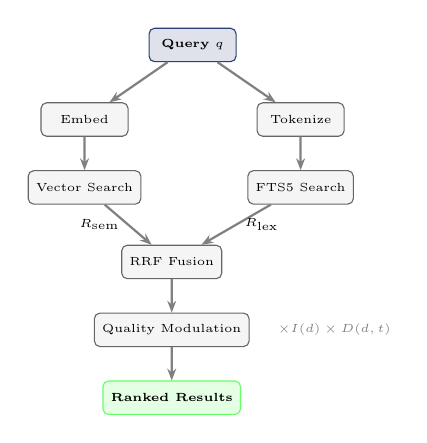
\begin{tikzpicture}[
    scale=0.85,
    transform shape,
    node distance=0.4cm,
    box/.style={rectangle, draw=black!60, fill=lightgray, rounded corners=2pt, minimum width=1.3cm, minimum height=0.5cm, font=\tiny},
    query/.style={rectangle, draw=headerblue, fill=headerblue!15, rounded corners=2pt, minimum width=1.3cm, minimum height=0.5cm, font=\tiny\bfseries},
    result/.style={rectangle, draw=green!60, fill=green!10, rounded corners=2pt, minimum width=1.5cm, minimum height=0.5cm, font=\tiny\bfseries},
    arrow/.style={-{Stealth[length=1.5mm]}, thick, draw=black!50}
]

\node[query] (q) {Query $q$};

\node[box, below left=0.6cm and 0.3cm of q] (embed) {Embed};
\node[box, below right=0.6cm and 0.3cm of q] (tokenize) {Tokenize};

\node[box, below=0.5cm of embed] (vec) {Vector Search};
\node[box, below=0.5cm of tokenize] (fts) {FTS5 Search};

\node[box, below right=0.6cm and -0.3cm of vec] (rrf) {RRF Fusion};

\node[box, below=0.5cm of rrf] (quality) {Quality Modulation};

\node[result, below=0.5cm of quality] (results) {Ranked Results};

\draw[arrow] (q) -- (embed);
\draw[arrow] (q) -- (tokenize);
\draw[arrow] (embed) -- (vec);
\draw[arrow] (tokenize) -- (fts);
\draw[arrow] (vec) -- node[left, font=\tiny] {$R_{\text{sem}}$} (rrf);
\draw[arrow] (fts) -- node[right, font=\tiny] {$R_{\text{lex}}$} (rrf);
\draw[arrow] (rrf) -- (quality);
\draw[arrow] (quality) -- (results);

\node[right=0.3cm of quality, font=\tiny, text=gray] {$\times I(d) \times D(d,t)$};

\end{tikzpicture}
\caption{Hybrid search pipeline. Queries undergo parallel lexical (FTS5) and semantic (vector) retrieval. Results merge via RRF, then modulate by quality signals.}
\label{fig:search-pipeline}
\end{figure}

\begin{definition}[Reciprocal Rank Fusion]
Given ranking functions $R_1, \ldots, R_m$, the RRF score for document $d$ is:
\begin{equation}
\text{RRF}(d) = \sum_{i=1}^{m} \frac{1}{k + \text{rank}_{R_i}(d)}
\end{equation}
where $k = 60$ is the smoothing constant \cite{cormack2009rrf}.
\end{definition}

For \yonakh\ with lexical ($R_{\text{lex}}$) and semantic ($R_{\text{sem}}$) retrieval:
\begin{equation}
\text{RRF}(d) = \frac{1}{60 + \text{rank}_{\text{lex}}(d)} + \frac{1}{60 + \text{rank}_{\text{sem}}(d)}
\end{equation}

The final relevance score incorporates quality:
\begin{equation}
\text{score}(d, q, t) = \text{RRF}(d) \cdot I(d) \cdot D(d, t)
\end{equation}

\textbf{Semantic Similarity.} Vector search uses cosine similarity:
\begin{equation}
\text{sim}(q, d) = \frac{\mathbf{v}_q \cdot \mathbf{v}_d}{\|\mathbf{v}_q\| \|\mathbf{v}_d\|}
\end{equation}
where $\mathbf{v}_q, \mathbf{v}_d \in \mathbb{R}^{384}$ are embeddings from a sentence transformer model.

\textbf{Lexical Scoring.} FTS5 uses BM25:
\begin{equation}
\text{BM25}(d, q) = \sum_{t \in q} \text{IDF}(t) \cdot \frac{f(t,d) \cdot (k_1 + 1)}{f(t,d) + k_1 \cdot (1 - b + b \cdot \frac{|d|}{\text{avgdl}})}
\end{equation}

\subsection{Rules Engine}

The rules engine automates relationship inference through a four-stage pipeline (Fig.~\ref{fig:rules-pipeline}).

\begin{figure}[t]
\centering
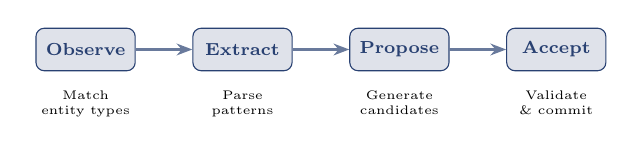
\begin{tikzpicture}[
    scale=0.9,
    transform shape,
    node distance=0.8cm,
    stage/.style={rectangle, draw=headerblue, fill=headerblue!15, rounded corners=3pt, minimum width=1.4cm, minimum height=0.6cm, font=\scriptsize\bfseries, text=headerblue},
    arrow/.style={-{Stealth[length=2mm]}, thick, draw=headerblue!70}
]

\node[stage] (observe) {Observe};
\node[stage, right=of observe] (extract) {Extract};
\node[stage, right=of extract] (propose) {Propose};
\node[stage, right=of propose] (accept) {Accept};

\draw[arrow] (observe) -- (extract);
\draw[arrow] (extract) -- (propose);
\draw[arrow] (propose) -- (accept);

\node[below=0.15cm of observe, font=\tiny, text width=1.4cm, align=center] {Match entity types};
\node[below=0.15cm of extract, font=\tiny, text width=1.4cm, align=center] {Parse patterns};
\node[below=0.15cm of propose, font=\tiny, text width=1.4cm, align=center] {Generate candidates};
\node[below=0.15cm of accept, font=\tiny, text width=1.4cm, align=center] {Validate \& commit};

\end{tikzpicture}
\caption{Rules engine pipeline. Rules observe specific entity types, extract patterns (e.g., issue references), propose relationships, and commit validated edges.}
\label{fig:rules-pipeline}
\end{figure}

Formally, a rule $\rho$ is a tuple:
\begin{equation}
\rho = (\mathcal{T}_{\text{obs}}, f_{\text{extract}}, f_{\text{propose}}, \theta_{\text{conf}})
\end{equation}
where $\mathcal{T}_{\text{obs}} \subseteq \mathcal{T}_V$ are observed types, $f_{\text{extract}}: V \to \mathcal{F}$ extracts findings, $f_{\text{propose}}: \mathcal{F} \to \mathcal{E}$ proposes edges, and $\theta_{\text{conf}}$ is the confidence threshold.

\textbf{Example: Git Rule.} For commits, the rule extracts:
\begin{align}
f_{\text{extract}}^{\text{git}}(e) = \{&\text{issue\_refs}(\phi(e)[\text{msg}]), \notag \\
&\text{adr\_refs}(\phi(e)[\text{msg}]), \\
&\text{revert\_refs}(\phi(e)[\text{msg}])\} \notag
\end{align}
and proposes edges like $(e, e_{\text{issue}}, \texttt{fixes})$.

\subsection{Provenance and Time-Travel}

Every modification generates a provenance record:
\begin{equation}
p = (\text{entity\_id}, \text{actor}, \text{action}, t, \Delta\text{conf}, \text{snapshot})
\end{equation}

This enables point-in-time queries. The state at time $t$ is:
\begin{equation}
G_t = \text{apply}(G_0, \{p : p.t \leq t\})
\end{equation}

\subsection{Integration Interfaces}

\yonakh\ exposes two complementary interfaces designed for different integration patterns.

\subsubsection{REST API}

The REST API provides standard HTTP endpoints following RESTful conventions:

\begin{itemize}
\item \textbf{Entity CRUD:} \texttt{POST/GET/PUT/DELETE /entities/\{id\}} for full lifecycle management with JSON payloads
\item \textbf{Relationship management:} \texttt{POST /relationships} to create typed edges between entities
\item \textbf{Search:} \texttt{POST /search} accepting query text, filters, and pagination parameters
\item \textbf{Provenance:} \texttt{GET /entities/\{id\}/history} returns the complete audit trail
\item \textbf{Time-travel:} \texttt{GET /snapshot?at=\{timestamp\}} reconstructs historical state
\item \textbf{Batch operations:} \texttt{POST /batch} for atomic multi-entity transactions
\end{itemize}

The REST API suits traditional integrations, CI/CD pipelines, and tools without MCP support. Authentication uses API keys with configurable scopes.

\subsubsection{Model Context Protocol (MCP) Server}

For AI coding assistants, \yonakh\ implements the Model Context Protocol \cite{mcp2024}---an emerging standard for tool-use interfaces. Table~\ref{tab:mcp} summarizes the ten MCP tools.

\begin{table}[t]
\caption{MCP Tool Specifications}
\label{tab:mcp}
\centering
\small
\renewcommand{\arraystretch}{1.3}
\begin{tabular}{@{}p{0.38\columnwidth} p{0.54\columnwidth}@{}}
\toprule
\textbf{Tool} & \textbf{Function} \\
\midrule
remember & Store entity with auto-typing \\
recall & Hybrid search with ranking \\
record\_decision & Create ADR-style decision \\
record\_failed\_attempt & Store negative knowledge \\
get\_context & Retrieve file context \\
find\_contradictions & Detect conflicts \\
link\_entities & Create relationship \\
time\_travel & Query past state \\
get\_provenance & Retrieve audit trail \\
search\_by\_type & Type-filtered search \\
\bottomrule
\end{tabular}
\end{table}

Any MCP-compatible tool can connect by adding a single configuration entry:

\begin{verbatim}
{"mcpServers": {"yonakh": {
  "command": "python",
  "args": ["-m", "yonakh.mcp_server"]}}}
\end{verbatim}

The MCP interface enables AI assistants to read and write memory as naturally as they read and write files, making memory operations a first-class capability rather than an afterthought.

\section{Usage Scenarios}

We present four scenarios illustrating how \yonakh\ addresses real development challenges. Each scenario describes the problem, the \yonakh-enabled workflow, and a concrete example.

\subsection{Scenario 1: Developer Onboarding}

\textbf{Problem:} New team members face a steep learning curve. Codebases accumulate implicit knowledge---why certain patterns were chosen, what alternatives were rejected, which areas are fragile---that exists only in the minds of senior developers or scattered across chat logs.

\textbf{Workflow:} When a new developer's AI assistant starts a session, it calls \texttt{get\_context} with the current working directory. \yonakh\ returns relevant decisions, design rationale, and known issues ranked by importance and recency. As the developer explores code, \texttt{recall} surfaces related knowledge. When they propose changes, \texttt{find\_contradictions} checks for conflicts with existing decisions.

\textbf{Example:} A new developer asks their AI assistant: ``Why are we using JWTs instead of server-side sessions?''

The assistant calls \texttt{recall("JWT session authentication decision")}. \yonakh\ returns:

\begin{quote}
\textbf{Decision:} Use JWT tokens for authentication (created 18 months ago, importance: 0.92)

\textbf{Context:} We needed to support horizontal scaling across multiple API servers without shared session state.

\textbf{Alternatives considered:} (1) Redis-backed sessions---rejected due to operational complexity and single point of failure; (2) Sticky sessions---rejected due to poor load distribution.

\textbf{Consequences:} Larger request headers, token refresh complexity, inability to invalidate tokens server-side without blacklist.

\textbf{Related:} Links to the PR implementing JWT auth, the security review, and a subsequent bug report about token expiry edge cases.
\end{quote}

The developer gains not just the \emph{what} but the \emph{why}---context that would otherwise require interrupting a senior colleague or archaeological digging through git history.

\subsection{Scenario 2: Debugging Knowledge Preservation}

\textbf{Problem:} Debugging sessions generate valuable knowledge---hypotheses tested, dead ends encountered, root causes discovered---that evaporates when the session ends. Teams repeatedly debug the same issues because negative knowledge (``we tried X and it didn't work because Y'') is never captured.

\textbf{Workflow:} During debugging, the AI assistant records hypotheses and outcomes. When a dead end is reached, \texttt{record\_failed\_attempt} captures what was tried and why it failed. When the root cause is found, a bug report entity links to the failed attempts and the fix. Future sessions querying similar symptoms retrieve this knowledge.

\textbf{Example:} A developer encounters intermittent API 500 errors under load. Their AI assistant calls \texttt{recall("API 500 errors load performance")}. \yonakh\ returns:

\begin{quote}
\textbf{Bug Report:} API 500 errors under sustained load (resolved 3 months ago)

\textbf{Root cause:} Database connection pool exhaustion due to leaked connections in error paths.

\textbf{Failed attempts:}
\begin{itemize}
\item Increased pool size from 20 to 50---masked symptoms temporarily but leak continued
\item Added connection timeout---helped but didn't address root cause
\item Suspected query performance---ruled out via profiling
\end{itemize}

\textbf{Actual fix:} Added \texttt{finally} blocks to ensure connection release in 3 error handlers (links to commit).

\textbf{Lesson:} Always check connection release in exception paths when seeing pool exhaustion.
\end{quote}

Instead of spending hours re-investigating, the developer immediately knows where to look and what approaches don't work.

\subsection{Scenario 3: Multi-Agent Coordination}

\textbf{Problem:} Development teams increasingly use multiple AI tools---one for coding, another for code review, another for documentation. Without shared context, these tools may give contradictory advice or miss important constraints.

\textbf{Workflow:} All AI agents connect to the same \yonakh\ instance. When the coding assistant records a decision, the review bot can see it. When the documentation assistant needs to explain a design choice, it can query the rationale. Agents coordinate through shared memory rather than requiring human intermediation.

\textbf{Example:} A developer uses Cursor to implement an async version of a previously synchronous API endpoint. They submit a PR. The review bot (running Claude) examines the changes and calls \texttt{recall("audit logging synchronous async payment")}. \yonakh\ returns:

\begin{quote}
\textbf{Decision:} Payment endpoints must use synchronous processing (created 8 months ago)

\textbf{Context:} Audit logging requires guaranteed ordering; async processing could interleave log entries from concurrent requests, making forensic analysis difficult.

\textbf{Constraint:} Applies to all endpoints in \texttt{/api/payments/*}
\end{quote}

The review bot flags the PR: ``This change converts a payment endpoint to async processing, which may conflict with the audit logging decision requiring synchronous processing for payment operations. Please verify this change is intentional and update the decision if the constraint no longer applies.''

The developer, the review bot, and the original decision author are all coordinated through \yonakh\ without explicit communication.

\subsection{Scenario 4: Architectural Evolution}

\textbf{Problem:} As systems evolve, architectural decisions become stale. What was the right choice two years ago may be wrong today. Teams need to track which decisions should be revisited and why.

\textbf{Workflow:} \yonakh's temporal decay naturally deprioritizes old decisions. The \texttt{find\_contradictions} tool surfaces decisions that conflict with recent changes. Periodic queries for high-importance, high-decay entities identify candidates for review.

\textbf{Example:} An architect queries: ``What architectural decisions should we revisit?''

The assistant calls \texttt{search\_by\_type("decision")} with filters for high importance but high decay (approaching half-life). \yonakh\ returns:

\begin{quote}
\textbf{Candidates for review:}
\begin{enumerate}
\item \textbf{Monolithic deployment} (age: 2.1 years, importance: 0.85, decay: 0.45)---Original rationale cited team size; team has tripled since then.

\item \textbf{PostgreSQL for all storage} (age: 1.8 years, importance: 0.82, decay: 0.52)---Recent feature requests suggest need for document store capabilities.

\item \textbf{No caching layer} (age: 1.5 years, importance: 0.78, decay: 0.61)---Traffic has grown 10x; original simplicity argument may no longer apply.
\end{enumerate}
\end{quote}

Each candidate links to the original decision, subsequent discussions, and related entities. The architect can make informed choices about which decisions to revisit based on how context has changed.

\section{Discussion}

\subsection{Implications for AI-Assisted Development}

\subsubsection{From Isolated Tools to Coordinated Ecosystems}

Current AI coding assistants operate as isolated tools, each with its own context window and no persistent memory. \yonakh\ transforms this landscape by providing a shared substrate that enables coordination without explicit integration. Tools that speak MCP can participate in a memory ecosystem simply by connecting to a \yonakh\ instance.

This has profound implications for tool composition. Instead of choosing a single ``best'' AI assistant, developers can use specialized tools for different tasks---one optimized for code generation, another for review, another for documentation---with \yonakh\ providing continuity across them.

\subsubsection{Organizational Memory for AI}

Knowledge management literature distinguishes individual from organizational memory \cite{walsh1991organizational}. Current AI assistants have only individual memory (their context window); when a session ends, organizational knowledge is lost. \yonakh\ provides organizational memory for AI systems, enabling:

\begin{itemize}
\item \textbf{Knowledge accumulation:} Insights compound across sessions rather than resetting
\item \textbf{Expertise distribution:} Knowledge from expert developers becomes accessible to all team members' AI assistants
\item \textbf{Institutional continuity:} When developers leave, their recorded decisions and rationale remain
\end{itemize}

\subsubsection{The Value of Negative Knowledge}

Software engineering research emphasizes learning from failure \cite{parnas1994software}, yet negative knowledge---what doesn't work and why---is rarely captured systematically. AI assistants frequently suggest approaches that experienced developers know are dead ends.

\yonakh's explicit modeling of \texttt{failed\_attempt} entities addresses this gap. By recording not just successes but failures, teams build a corpus of ``don't do this because...'' knowledge that prevents AI assistants from repeatedly suggesting ineffective solutions.

\subsubsection{Temporal Coherence in Knowledge Systems}

Unlike static documentation, software knowledge has temporal dynamics. A decision made two years ago under different constraints may be actively harmful today. \yonakh's decay model ensures that recent knowledge is prioritized while old knowledge remains accessible but appropriately discounted.

This temporal awareness enables proactive knowledge maintenance: entities approaching their half-lives surface for review, preventing the accumulation of stale guidance that plagues traditional documentation systems.

\subsection{Limitations and Threats to Validity}

\subsubsection{Cold Start Problem}

New \yonakh\ deployments contain no knowledge. Value accrues over time as teams record decisions and the rules engine infers relationships. We mitigate this through:

\begin{itemize}
\item \textbf{Git history import:} Automatically creating entities from commit messages, PRs, and issues
\item \textbf{Document ingestion:} Parsing existing ADRs and documentation
\item \textbf{Conversation mining:} Extracting decisions from chat logs (with appropriate permissions)
\end{itemize}

However, the richest knowledge---design rationale, failed attempts, tacit constraints---must be captured through ongoing use.

\subsubsection{Quality Calibration}

The importance weights and decay half-lives in \yonakh\ are based on domain intuition and informal feedback rather than rigorous empirical validation. Different teams, domains, and project phases may require different parameters. We provide configuration options but acknowledge that optimal values remain an open research question.

\subsubsection{Scalability}

The current SQLite implementation targets small-to-medium teams (up to ~50 developers, ~100K entities). Larger deployments would require:

\begin{itemize}
\item Migration to PostgreSQL or distributed databases
\item Sharding strategies for multi-team organizations  
\item Caching layers for high-frequency queries
\item Async processing for computationally expensive operations
\end{itemize}

We view the current implementation as a proof of concept; production deployments at scale would require additional engineering.

\subsubsection{Knowledge Correctness}

\yonakh\ stores knowledge without verifying its accuracy. If an AI assistant records an incorrect decision or a developer misattributes a bug's root cause, that misinformation persists and propagates. We partially address this through:

\begin{itemize}
\item \textbf{Provenance tracking:} Every entity records its source, enabling credibility assessment
\item \textbf{Conflict detection:} Contradictory entities surface for human resolution
\item \textbf{Decay:} Incorrect knowledge naturally loses influence over time if not reinforced
\end{itemize}

However, systematic verification of stored knowledge remains future work.

\subsubsection{Privacy and Security}

Shared memory raises privacy concerns. Sensitive information recorded in one session becomes accessible to others. \yonakh\ supports access control at the entity level, but organizations must establish policies about what knowledge should be shared versus kept private.

\subsection{Future Work}

Several directions warrant further investigation:

\textbf{Empirical evaluation:} Controlled studies measuring the impact of shared memory on developer productivity, onboarding time, and defect rates.

\textbf{Automatic knowledge extraction:} Using LLMs to automatically identify and record decisions from code changes, conversations, and documents without explicit user action.

\textbf{Cross-repository knowledge:} Extending \yonakh\ to share knowledge across related repositories, enabling organizational knowledge graphs.

\textbf{Confidence calibration:} Learning optimal importance weights and decay rates from usage patterns and feedback.

\textbf{Knowledge verification:} Techniques for validating stored knowledge against code reality and detecting drift.

\section{Conclusion}

The proliferation of AI coding assistants creates an unprecedented opportunity for augmented software development---and an unprecedented risk of knowledge fragmentation. Each tool generates valuable insights that evaporate between sessions and remain invisible to other tools. The result is a form of collective amnesia where organizations continuously create and lose engineering knowledge.

\yonakh\ addresses this challenge with a shared memory architecture grounded in both practical engineering and theoretical foundations:

\begin{itemize}
\item A \textbf{domain ontology} of 21 entity types and 21 relationship types captures the full spectrum of software engineering knowledge, from architectural decisions to failed debugging attempts.

\item A \textbf{memory quality model} formalizes knowledge lifecycle through multi-signal importance scoring, temporal decay with domain-specific half-lives, and automated conflict detection.

\item An \textbf{open architecture} via REST API and Model Context Protocol enables any tool to participate in the shared memory ecosystem without custom integration.

\item A \textbf{theoretical foundation} in cognitive science and knowledge management explains why shared, quality-aware memory should improve AI-assisted development outcomes.
\end{itemize}

We have presented the design, formalization, and usage scenarios for \yonakh. The system is implemented and available as open-source software at \url{https://github.com/shvenkat/yonakh}. While empirical validation remains future work, we believe the architecture addresses a fundamental gap in current AI-assisted development tooling.

As AI becomes increasingly central to software development, shared memory may emerge as important infrastructure for effective human-AI collaboration. Just as version control became indispensable for coordinating code changes, memory systems like \yonakh\ could play a similar role for coordinating AI-generated knowledge. We offer this work as a step toward exploring that possibility.

\bibliographystyle{IEEEtran}
\bibliography{references}

\end{document}
